%Alignment Process in Metashape
%tikzstyle
\tikzstyle{decision} = [diamond, draw, fill=blue!20, 
text width=6em, text badly centered, node distance=3cm, inner sep=0pt]
\tikzstyle{block} = [rectangle, draw, fill=blue!20, 
text width=6em, text centered, rounded corners, minimum height=2em]
\tikzstyle{block2} = [rectangle, draw, fill=yellow!20, 
text width=9em, text centered, rounded corners, minimum height=4em]
\tikzstyle{line} = [draw, -latex']
\tikzstyle{cloud} = [draw, ellipse,fill=red!20, node distance=3cm,
minimum height=4em]


\paragraph{Alignment}
\label{alignment}

The alignment is the first step in the reconstruction process in agisoft metashape. This step can be broken down into different stages when we reconstruct the region of intrest.
\begin{figure}[!ht]
	\centering
	\begin{tikzpicture}[node distance = 2cm, auto]
		\node [block] (init) {selection of images};
		\node [block, right of = init, node distance = 4cm] (mask) {applying masks};
		\node [block, right of = mask, node distance = 4cm] (markers) {placing markers};
		\node [block, right of = markers, node distance = 4cm] (alignment) {alignment of images};
		\path [line] (init) -- (mask);
		\path [line] (mask) -- (markers);
		\path [line] (markers) -- (alignment);
	\end{tikzpicture}
	\label{pipe:alignment}
	\caption{alignment process}
\end{figure}
\subparagraph{selection of images}
\label{selectionofimages}

In our project we selected the images based on the most visited location by the rover and the amount of time that the rover has spent on that particular region. We decided the region based on the information \cite{locationMap} provided by NASA. By calculating the sols we can infer the number of days the rover has spent on a region from which we can choose a particular range of sols to reconstruct. Since the \cite{pdsNode} contains a plethora of images which will include the claibration target, on-board equipments, images of sun, test images, etc. It will become a tedious process to Identity the images from each sol that can provide us with a good model in the final stages since downloading multiple sols consumes lot of time and at some sols not all images will be required for the reconstruction. We used the \cite{stereoImages} to filter the sols that have good images for the reconstruction. From our work with Agisoft metashape we infered that for a good reconstruction we should provide the images from different views for a single object/rock. So we selected locations that had multiple images form different angles.

\subparagraph{Applying Masks}
\label{applyingMasks}

Metashape provides a tool with which we can mask the unwanted noise/background in the images. We used this feature since somes images had a good description of the object to be reconstructed but hindered by other objects, rover equipments, etc. 

\subparagraph{Placing Markers}
\label{placingMarkers}

Markers are used to interlink one point in a image with another image. This speeds up the alignment process and also points agisoft to align the images based on the markers. Thus by connecting multiple images with the markers we will be able ot get a good reconstruction from the selected images.

\begin{figure}[H]
	\centering
	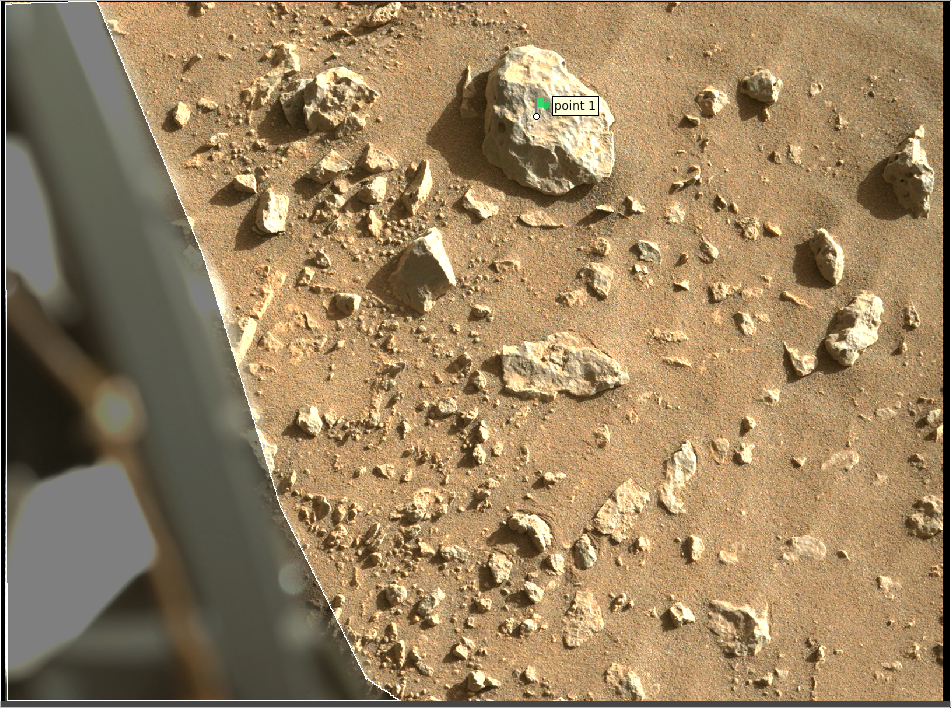
\includegraphics[scale=0.3]{img/masksandMarkers.png}
	\caption{Applying Masks and Markers}
	\label{fig:masksMarkers}
\end{figure}
\subparagraph{Alignment of Images}
\label{alignmentOfImages}
This step performs triangulation and bundle block adjustment. Agisoft searches for feature points across the images and matches them to tie points. It estimates the camera position of each image, also with the intrinsic and the extrinsic camera parameters.\emph{Masks} and \emph{Markers} allows agisoft to searche for feature points in those specific regions. This allows us to ignore the unessential parts for the reconstruction as we work with different cameras with distinct characteristics. While aligning we used the high accurarcy settings and increased the keypoint limit to 40,00. Increasing the accurarcy may provide better results but the time for the alignment will be considerably increased.
\begin{figure}[H]
	\centering
	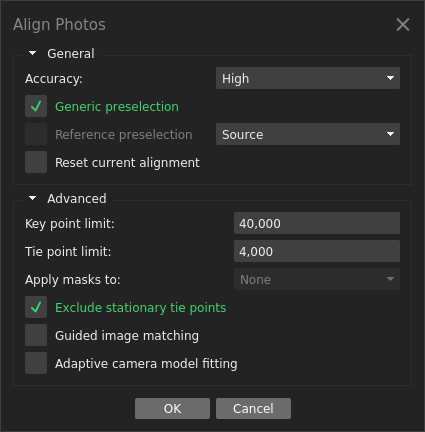
\includegraphics[scale=0.6]{img/alignmet.png}
	\caption{Alignment in Agisoft}
	\label{fig:alignment}
\end{figure}
The output of the alignment process gives the tie points and a set of estimated camera positions. The result of alignment will be determined by the number of images that have been fully aligned as some images tend not to align. The tie points represents the results of the image alignment and also used for the determination of the depth map calculation 

